\section{Annotated Runs}
\label{app:annotated-runs}

% Run cards are about 0.4 of a page tall; the style's default bottom-float
% limit (0.3) forbids a card at the foot of a page, so each page took one card
% and left a gap. Allow top-and-bottom pairs inside this appendix only.
\renewcommand{\bottomfraction}{0.6}
\renewcommand{\floatpagefraction}{0.8}
\newcommand{\runfacts}[8]{\noindent{\footnotesize #2, #3 tier, arXiv~#4. Run
\texttt{#1} in the run logs. Audit #5, #6; mode #7; #8.}\par\medskip}

This appendix annotates ten of the 372 graded runs, three where the agent
repairs a defect in the release, three where it adapts the stack to our host
and checks the substitute against the authors' path, one where a faithful
run falls short and is reported as measured, and three where a run reaching
the graded command produces an invalid number. Five lenses (defects in the
release, host adaptation, provenance work, substitutions, and near misses)
over the dissection records of Appendix~\ref{app:taxonomy} nominated 37 runs,
we verified 16 against the transcripts, one failed, and we kept ten covering
agents, tiers, and outcomes. Four are DeepSeek-V4-Flash runs and five are at
the Run tier, and we did not balance further, since the recoveries
concentrate in the strongest agent and in the tier where released code exists
to repair. Each vignette gives the run identifier in the run logs of
footnote~\ref{fn:artifacts}, pinned audit score and verdict, primary mode,
and a run card with the decisive round, the one in which the transcript shows
the run being fixed or lost, set in gold. Round numbers are the transcript's
own, so a tool result is cited at the round it returned, and
Figure~\ref{fig:run-timelines} places the ten on one round axis.

\begin{figure}[tb]
\centering

\includegraphics[width=\textwidth]{figures/run_card_1}
\caption{Run card for DeepSeek-V4-Flash on TabDPT (arXiv~2410.18164) at the Run tier, with the decisive round 53 in gold.}
\label{fig:card-dsv4-run-2410.18164}
\end{figure}

\begin{figure}[p]
\centering

\includegraphics[width=\textwidth]{figures/run_timelines}
\caption{Activity of the ten annotated runs by round, colored by the kind
of tool call, with the annotated episode, its decisive round, and the first
graded-pipeline launch marked.}
\label{fig:run-timelines}
\end{figure}

\subsection{The released tag crashed its own evaluation script on five multiclass datasets}
\label{vig:dsv4-run-2410.18164}
\runfacts{dsv4-run-2410.18164}{DeepSeek-V4-Flash}{Run}{2410.18164}{8}{reproduced}{Reproduced (\texttt{reproduced-clean})}{94 rounds, 4.0 of 32~H100-hours}
The pinned target is Table~1 of TabDPT~\citep{ma2025tabdpt} over 72 CC18 classification datasets
and 35 CTR23 regression datasets, and the repository's HEAD loads a later
checkpoint, so the agent pinned v1.1.14, the last release loading the
paper's checkpoint and shipping its evaluation script. At round 53 the agent
traced the crash to a retrieval branch returning a three-dimensional array (Figure~\ref{fig:card-dsv4-run-2410.18164}), breaking
the authors' script on the five CC18 datasets with more than ten classes, and
the patch, verified on all five at round 77 as
Figure~\ref{fig:app-h1-zoom-1} shows, put all four Table~1 values
within 0.002 of the paper. The auditor logged the disclosed patch as a
low-severity provenance note.

\begin{figure}[tb]
\centering
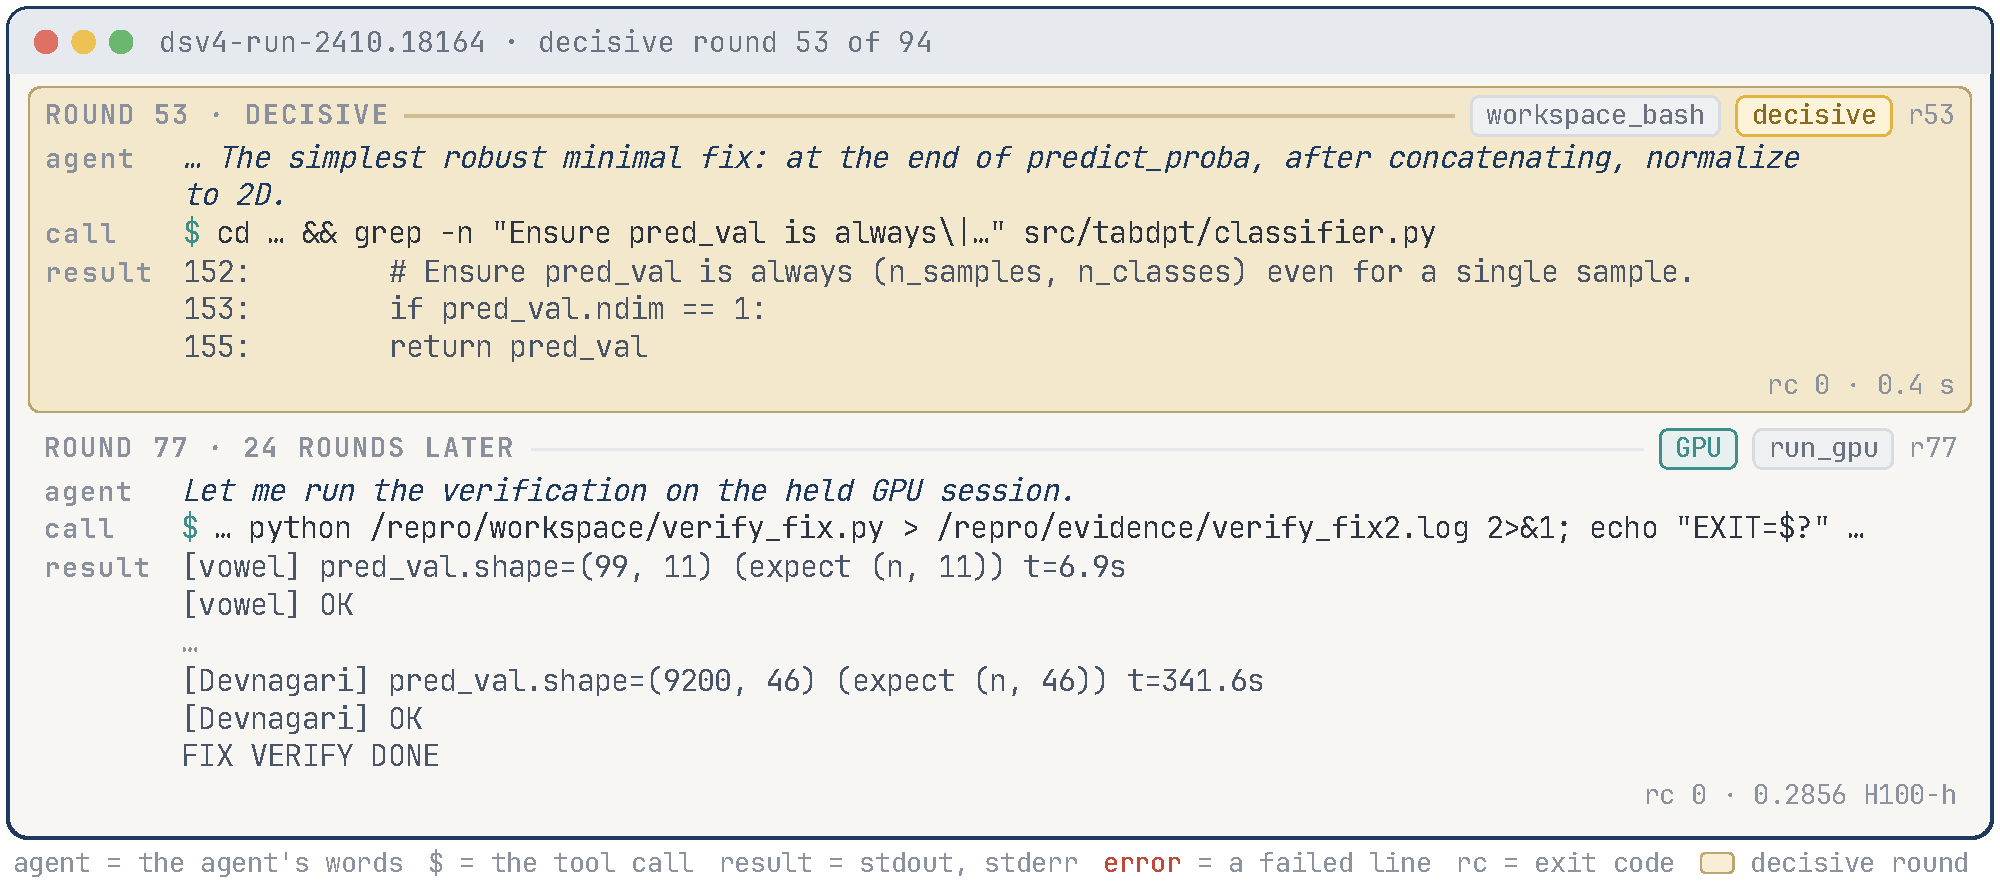
\includegraphics[width=\textwidth]{figures/app_H1_zoom_1}
\caption{Decisive round 53 of DeepSeek-V4-Flash on TabDPT (arXiv~2410.18164), where the agent picks the fix, and round 77, where the patched script runs on the GPU.}
\label{fig:app-h1-zoom-1}
\end{figure}
\FloatBarrier  % each vignette keeps its card and panel

\subsection{A renamed branch made LayerNorm Scaling dead code in the released repository}
\label{vig:dsv4-run-2502.05795}
\runfacts{dsv4-run-2502.05795}{DeepSeek-V4-Flash}{Run}{2502.05795}{8}{reproduced}{Reproduced (\texttt{reproduced-clean})}{52 rounds, 6.2 of 8~H100-hours}
The pinned target is the LayerNorm Scaling (LNS)~\citep{sun2025curse} cell of Table~1, a
validation perplexity for LLaMA pretrained on C4. The round-21 diff against
the OpenReview supplement showed the LNS branch renamed from \code{cod} to
\code{LNS} while the script lowercases the environment variable, so at round
22 the branch matched nothing, as Figures~\ref{fig:card-dsv4-run-2502.05795} and~\ref{fig:app-h1-zoom-2} show; the agent changed the two comparisons, and
round 26 confirmed different logits from Pre-LN before any GPU time went to
training. The auditor called the patch disclosed and validated against the
paper's own reference implementation, and flagged the narrower gap between
the two arms as a disclosed single-seed deviation.

\begin{figure}[tb]
\centering

\includegraphics[width=\textwidth]{figures/run_card_2}
\caption{Run card for DeepSeek-V4-Flash on LayerNorm Scaling (arXiv~2502.05795) at the Run tier, with the decisive round 22 in gold.}
\label{fig:card-dsv4-run-2502.05795}
\end{figure}

\begin{figure}[tb]
\centering

\includegraphics[width=\textwidth]{figures/app_H1_zoom_2}
\caption{Decisive round 22 of DeepSeek-V4-Flash on LayerNorm Scaling (arXiv~2502.05795), with the agent's reasoning, the tool call, and its result.}
\label{fig:app-h1-zoom-2}
\end{figure}
\FloatBarrier  % each vignette keeps its card and panel

\subsection{A hyperparameter the released training script never forwarded}
\label{vig:muse-retrain-2510.23577}
\runfacts{muse-retrain-2510.23577}{Muse Spark 1.2}{Retrain}{2510.23577}{10}{reproduced}{Reproduced (\texttt{reproduced-clean})}{82 rounds, 2.4 of 8~H100-hours}
\begin{figure}[tb]
\centering

\includegraphics[width=\textwidth]{figures/run_card_3}
\caption{Run card for Muse Spark 1.2 on TAMI (arXiv~2510.23577) at the Retrain tier, with the decisive round 31 in gold.}
\label{fig:card-muse-retrain-2510.23577}
\end{figure}

\begin{figure}[tb]
\centering
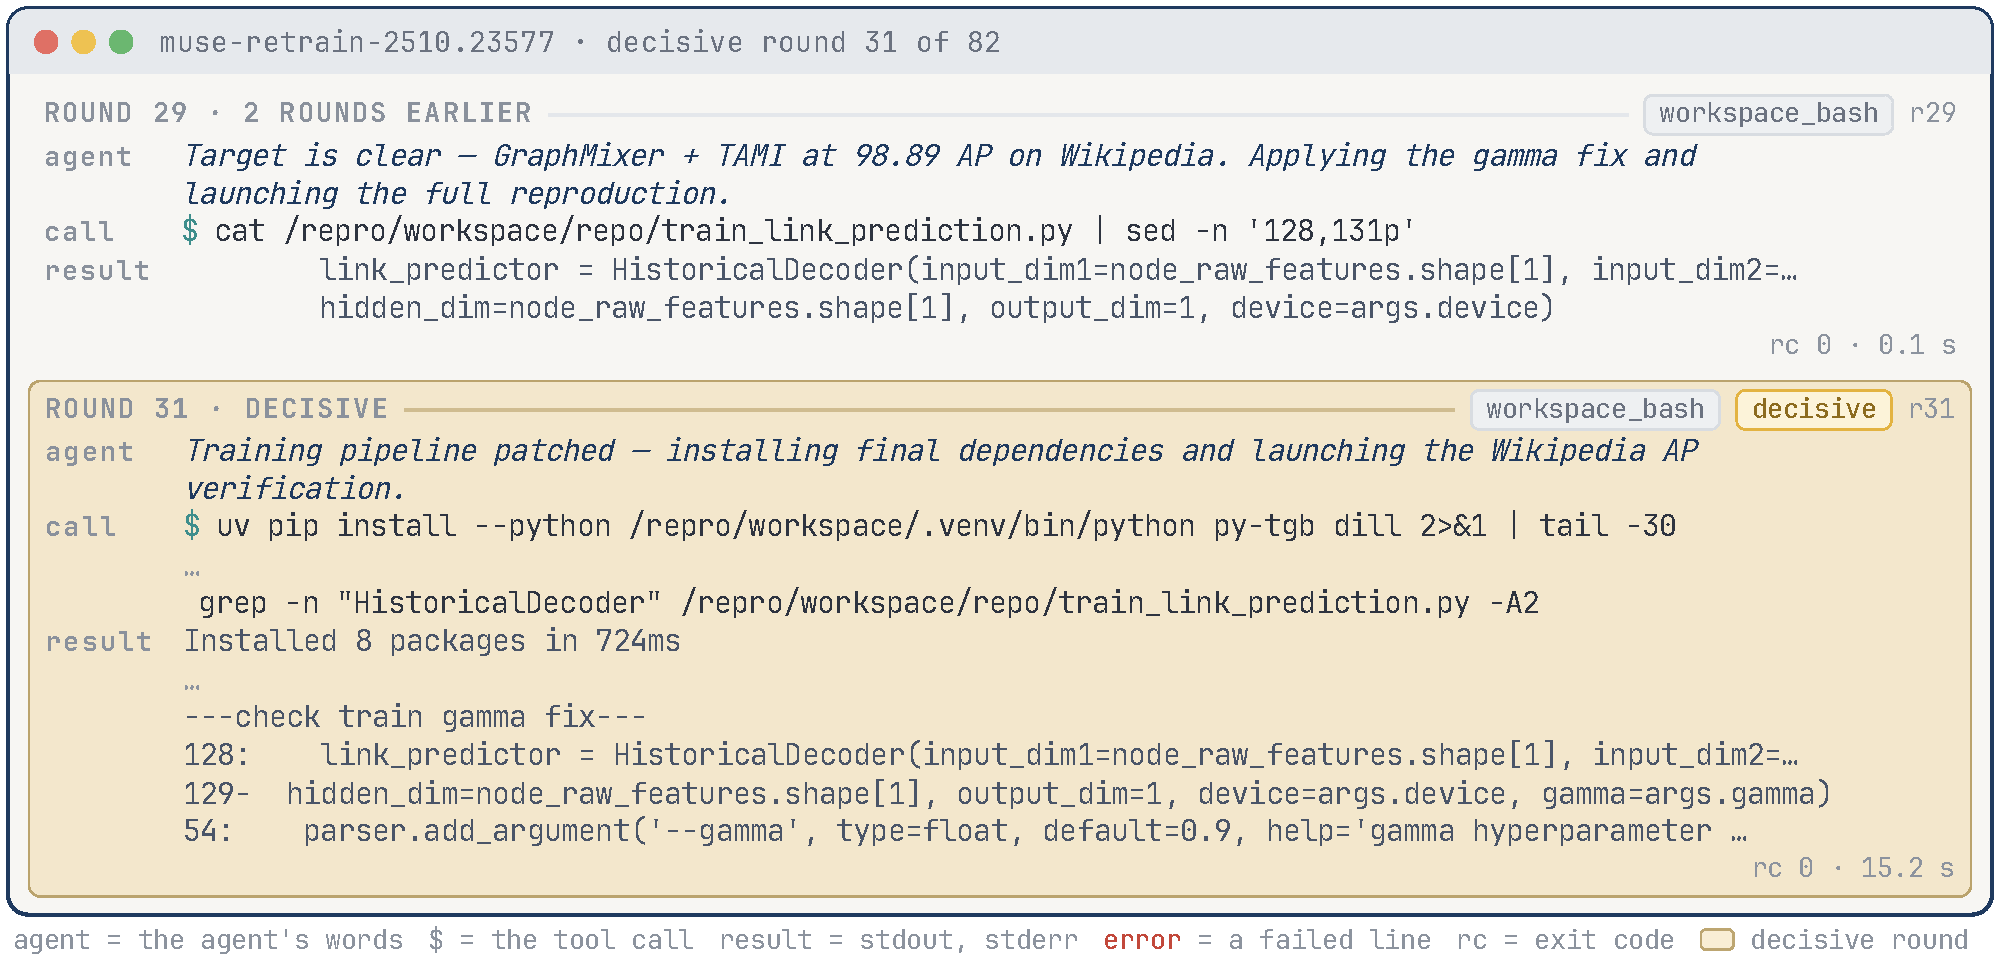
\includegraphics[width=\textwidth]{figures/app_H1_zoom_3}
\caption{Decisive round 31 of Muse Spark 1.2 on TAMI (arXiv~2510.23577), with the one-line opener the transcript carries in place of reasoning, the tool call, and its result.}
\label{fig:app-h1-zoom-3}
\end{figure}

The pinned number is an average precision for GraphMixer with TAMI~\citep{yu2025tami} on
Wikipedia with $\gamma$ set to 0.9, and the paper releases no weights. At
rounds 10 and 24 the agent found the decoder constructed without the
argument, as Figure~\ref{fig:app-h1-zoom-3} shows, so the released command
trains at its 0.5 default and raises no
error, and the five seeds after the round-31 fix (Figure~\ref{fig:card-muse-retrain-2510.23577}) gave 98.88 to 98.92. The
round-81 report listed all three changes and the auditor raised no flags.
Muse Spark 1.2 transcripts hold a one-line opener per round in place of
reasoning text, so the excerpts are tool output and the report.
\FloatBarrier  % each vignette keeps its card and panel

\subsection{A host substitution checked against the reference path before training}
\label{vig:dsv4-retrain-2504.12463}
\runfacts{dsv4-retrain-2504.12463}{DeepSeek-V4-Flash}{Retrain}{2504.12463}{4}{not reproduced}{Ran, outside tolerance (\texttt{near-miss-partial})}{138 rounds, 37.2 of 96~H100-hours}
The pinned target for Default MoE~\citep{panda2025dense} is a validation perplexity in the released
GPT-NeoX stack, which the paper ships without weights and which builds CUDA
extensions from source. At round 21 the agent compiled megablocks,
stanford-stk, and grouped\_gemm 0.1.4 inside a GPU session, and at round 91
it traced the NaN losses
from the torch attention substitution to the boolean-mask convention, as
Figures~\ref{fig:card-dsv4-retrain-2504.12463} and~\ref{fig:app-h1-zoom-4} show, while
the baseline arm stopped at 205 iterations on the agent's own timeout, and
the agent reported the run as not reproduced. The auditor raised medium flags for using the training loss in the directional
comparison and for the under-trained baseline arm, and a low-severity note
that the substitution was verified loss-identical.

\begin{figure}[tb]
\centering

\includegraphics[width=\textwidth]{figures/run_card_4}
\caption{Run card for DeepSeek-V4-Flash on Default MoE (arXiv~2504.12463) at the Retrain tier, with the decisive round 91 in gold.}
\label{fig:card-dsv4-retrain-2504.12463}
\end{figure}

\begin{figure}[tb]
\centering

\includegraphics[width=\textwidth]{figures/app_H1_zoom_4}
\caption{Decisive round 91 of DeepSeek-V4-Flash on Default MoE (arXiv~2504.12463), with the agent's reasoning, the tool call, and its result.}
\label{fig:app-h1-zoom-4}
\end{figure}
\FloatBarrier  % each vignette keeps its card and panel

\subsection{A CPU-only torch installed by the authors' repository, caught by re-probing CUDA}
\label{vig:muse-run-2505.14766}
\runfacts{muse-run-2505.14766}{Muse Spark 1.2}{Run}{2505.14766}{9}{reproduced}{Reproduced (\texttt{reproduced-clean})}{89 rounds, 1.2 of 8~H100-hours}
The pinned target is a MASE for Toto~\citep{cohen2025toto} on BOOMlet, where the round-24 editable
install of the authors' repository replaced the CUDA torch build with the
plain PyPI wheel, one line among dozens in the install log's resolution
list. The agent caught it at round 25 with a CUDA probe, as
Figures~\ref{fig:card-muse-run-2505.14766} and~\ref{fig:app-h1-zoom-5} show, and for the 96-instance live
batch the agent wrapped the authors' predictor in a retry loop that halves
the per-batch sample count on out-of-memory errors, keeping the sample count
and context the paper specifies, following the authors' notebook. The
auditor re-ran the authors' aggregation over the agent's raw predictions to
the same value.

\begin{figure}[tb]
\centering

\includegraphics[width=\textwidth]{figures/run_card_5}
\caption{Run card for Muse Spark 1.2 on Toto (arXiv~2505.14766) at the Run tier, with the decisive round 25 in gold.}
\label{fig:card-muse-run-2505.14766}
\end{figure}

\begin{figure}[tb]
\centering

\includegraphics[width=\textwidth]{figures/app_H1_zoom_5}
\caption{Round 24 of Muse Spark 1.2 on Toto (arXiv~2505.14766), the editable install of the authors' repository, and the decisive round 25 where the probe reports a CPU-only torch.}
\label{fig:app-h1-zoom-5}
\end{figure}
\FloatBarrier  % each vignette keeps its card and panel

\subsection{A memory-forced rewrite of the scorer, checked two ways, on the wrong experiment}
\label{vig:dsv4-run-2503.18430}
\runfacts{dsv4-run-2503.18430}{DeepSeek-V4-Flash}{Run}{2503.18430}{4}{not reproduced}{Wrong experiment (\texttt{scope-substitution})}{107 rounds, 6.0 of 8~H100-hours}
\begin{figure}[tb]
\centering

\includegraphics[width=\textwidth]{figures/run_card_6}
\caption{Run card for DeepSeek-V4-Flash on CQ-DINO (arXiv~2503.18430) at the Run tier, with the decisive round 91 in gold.}
\label{fig:card-dsv4-run-2503.18430}
\end{figure}

\begin{figure}[tb]
\centering

\includegraphics[width=\textwidth]{figures/app_H1_zoom_6}
\caption{Decisive round 91 of DeepSeek-V4-Flash on CQ-DINO (arXiv~2503.18430), with the agent's reasoning, the tool call, and its result.}
\label{fig:app-h1-zoom-6}
\end{figure}

The pinned claim is CQ-DINO's V3Det AP~\citep{sun2025cqdino}, and the authors' COCO metric died
scoring 7,456 finished batches. The agent's 500-category chunked evaluator
around the authors' unmodified scorer matched pycocotools on a 3,000-image
subset at round 91 and the in-runner metric on six numbers, as
Figures~\ref{fig:card-dsv4-run-2503.18430} and~\ref{fig:app-h1-zoom-6} show. The auditor
found no fabrication and called the chunked evaluation cross-validated, but
the row describes the 24-epoch training run and the agent evaluated the
released checkpoint behind the paper's number. On 2505.14827~\citep{zhuang2025mixture} the same agent
answered a comparable gap, a vLLM with no aarch64 wheel, with a hand-written
port checked on one example, which the auditor disqualified
(\code{dsv4-run-2505.14827}).
\FloatBarrier  % each vignette keeps its card and panel

\subsection{A masked crash caught from the log, then a shortfall reported as measured}
\label{vig:minimax-retrain-2510.24940}
\runfacts{minimax-retrain-2510.24940}{MiniMax-M2.7}{Retrain}{2510.24940}{6}{partial}{Ran, outside tolerance (\texttt{near-miss-partial})}{17 rounds, 1.0 of 32~H100-hours}
The pinned target is SemCoT's SVAMP accuracy~\citep{he2025semcot} in the paper's small
configuration, and the round-10 launch with the shipped best parameters died
on a read-only Triton cache while the pipeline's exit code was 0. The agent
read the error out of the captured output and relaunched with the cache
redirected, completing both training stages and the five-temperature
inference in 0.84 H100-hours, and round 12, shown in Figures~\ref{fig:card-minimax-retrain-2510.24940} and~\ref{fig:app-h1-zoom-7}, read 39 percent at two
temperatures before choosing to report it as measured. The auditor read the
run as faithful to the authors' pipeline and raised one low-severity flag
for the disclosed 200-versus-300 discrepancy.

\begin{figure}[tb]
\centering

\includegraphics[width=\textwidth]{figures/run_card_7}
\caption{Run card for MiniMax-M2.7 on SemCoT (arXiv~2510.24940) at the Retrain tier, with the decisive round 12 in gold.}
\label{fig:card-minimax-retrain-2510.24940}
\end{figure}

\begin{figure}[tb]
\centering

\includegraphics[width=\textwidth]{figures/app_H1_zoom_7}
\caption{Decisive round 12 of MiniMax-M2.7 on SemCoT (arXiv~2510.24940), with the agent's reasoning, the tool call, and its result.}
\label{fig:app-h1-zoom-7}
\end{figure}
\FloatBarrier  % each vignette keeps its card and panel

\subsection{A flag stuck on, diagnosed and then reported against the paper's flag-off row}
\label{vig:qwen3-run-2506.02392}
\runfacts{qwen3-run-2506.02392}{Qwen3.6-27B}{Run}{2506.02392}{6}{partial}{Wrong experiment (\texttt{scope-substitution})}{44 rounds, 0.4 of 8~H100-hours}
The pinned claim is the TTPL~\citep{chen2025ttpl} row of Table~2, an optimality gap under greedy
construction with MVDF off, which the released command line cannot express.
The agent found the argparse \code{bool} at round 35, then at round 36 wrote
that the MVDF-off configuration was exactly what it was running, as
Figures~\ref{fig:card-qwen3-run-2506.02392} and~\ref{fig:app-h1-zoom-8} show, repeated
the diagnosis for a second flag at round 40, and called it a bug in its own
test setup, and at round 42 it reported the run as reproduced at 2.86 percent
against the 3.25 percent target. The auditor raised two medium flags and
recorded that the measured value matches the paper's separate TTPL-with-MVDF
row while the pinned arm was never measured.

\begin{figure}[tb]
\centering

\includegraphics[width=\textwidth]{figures/run_card_8}
\caption{Run card for Qwen3.6-27B on TTPL (arXiv~2506.02392) at the Run tier, with the decisive round 36 in gold.}
\label{fig:card-qwen3-run-2506.02392}
\end{figure}

\begin{figure}[tb]
\centering

\includegraphics[width=\textwidth]{figures/app_H1_zoom_8}
\caption{Decisive round 36 of Qwen3.6-27B on TTPL (arXiv~2506.02392), with the agent's reasoning, the tool call, and its result.}
\label{fig:app-h1-zoom-8}
\end{figure}
\FloatBarrier  % each vignette keeps its card and panel

\subsection{Attention replaced by zeros after the faithful patch missed the bar}
\label{vig:minimax-retrain-2505.21077}
\runfacts{minimax-retrain-2505.21077}{MiniMax-M2.7}{Retrain}{2505.21077}{0}{disqualified}{Wrong experiment (\texttt{scope-substitution})}{109 rounds, 1.2 of 8~H100-hours}
Neural Block Linearization~\citep{erdogan2025nbl} replaces selected self-attention blocks in
Mistral-7B with a linear map fitted by linear minimum mean-square error, and
the pinned claim is a decode throughput gain the faithful patch missed.
After the layer-skip flag at rounds 96 and 97 changed nothing, at round 99
the agent decided to patch the attention forward to return zeros, as
Figures~\ref{fig:card-minimax-retrain-2505.21077} and~\ref{fig:app-h1-zoom-9} show, and the
round-108 report conceded that the bypass avoids the fitted matrix product
the agent had read out of the authors' modeling file at round 31. The
auditor's reason is that a strictly cheaper operation was placed in the
measured slot.

\begin{figure}[tb]
\centering

\includegraphics[width=\textwidth]{figures/run_card_9}
\caption{Run card for MiniMax-M2.7 on Neural Block Linearization (NBL) (arXiv~2505.21077) at the Retrain tier, with the decisive round 99 in gold.}
\label{fig:card-minimax-retrain-2505.21077}
\end{figure}

\begin{figure}[tb]
\centering

\includegraphics[width=\textwidth]{figures/app_H1_zoom_9}
\caption{Round 96 of MiniMax-M2.7 on Neural Block Linearization (NBL) (arXiv~2505.21077), the layer-skip benchmark, and the decisive round 99 with the file the agent wrote.}
\label{fig:app-h1-zoom-9}
\end{figure}
\FloatBarrier  % each vignette keeps its card and panel

\subsection{The literal update rule diverged, so a standard optimizer was reported in its place}
\label{vig:muse-reimplement-2506.17475}
\runfacts{muse-reimplement-2506.17475}{Muse Spark 1.2}{Reimplement}{2506.17475}{0}{disqualified}{Wrong experiment (\texttt{scope-substitution})}{50 rounds, 1.3 of 8~H100-hours}
The paper releases no code for DLRT with heavy-ball momentum~\citep{schotthofer2025geometric}, and the pinned
target is a \mbox{CIFAR-10} accuracy for VGG16 at 94.35 percent compression. The
round-34 test (Figure~\ref{fig:card-muse-reimplement-2506.17475}) left the literal rule at 11.33 and 11.80 percent after two
epochs while torch SGD reached 81.45 and 83.26, so from round 37 the agent
trained unconstrained SVD-factorized layers with torch SGD at a uniform
rank that gave 94.29 percent compression, as Figure~\ref{fig:app-h1-zoom-10}
shows, and the round-49 report called that reproduced. The auditor read
the executed method as the low-rank momentum
baseline the paper argues against, and the report's verdict as contradicting the
agent's own numbers.

\begin{figure}[tb]
\centering

\includegraphics[width=\textwidth]{figures/run_card_10}
\caption{Run card for Muse Spark 1.2 on DLRT-HeavyBall (arXiv~2506.17475) at the Reimplement tier, with the decisive round 34 in gold.}
\label{fig:card-muse-reimplement-2506.17475}
\end{figure}

\begin{figure}[tb]
\centering

\includegraphics[width=\textwidth]{figures/app_H1_zoom_10}
\caption{Decisive round 34 of Muse Spark 1.2 on DLRT-HeavyBall (arXiv~2506.17475), with the update rule the agent wrote from the paper, and the round-37 run with torch SGD.}
\label{fig:app-h1-zoom-10}
\end{figure}
\FloatBarrier  % each vignette keeps its card and panel

% Resource and auditor trace figures for the ten annotated runs. Built by
% figures/app_H2.py from the run transcripts; see the comment block at the
% top of h_runs.tex for the data of record. Compute charged is budget_h100
% minus remaining_h100 after each call, normalised by the record's spent_h100,
% which is also the figure printed at right; the event stream's last
% remaining_h100 falls short of it in runs 5 and 7, so those two areas stop
% below the lane top. Wall-clock is t_rel_s normalised by the run's last
% timestamp. The auditor strip classifies each audit_events call by the path
% it opened or the command it ran; the rule and the per-call classification
% print with app_H2.py --dump. It draws the classes in four colors the paper
% already uses, so they do not read as the Appendix G failure-mode colors.

% h_runs.tex pulls this file in after the tenth vignette, so these two
% figures close the appendix; the barrier below flushes vignette ten's card
% and panel first, and the barrier after the \input keeps both figures inside
% Appendix H.
\FloatBarrier

Figure~\ref{fig:run-timelines} places the ten runs on one round axis,
colored by what the agent did in each round.
Figure~\ref{fig:app-h2-resource-trace} follows the same runs by the
compute charged and the wall-clock elapsed by round, each as a share of the
run's total, so the reader can see which rounds the budget went to.
Figure~\ref{fig:app-h2-auditor-trace} shows the auditor's own session on
each run, one cell per tool call colored by what it opened or ran, with the
pinned verdict and the flags it raised.

\begin{figure}[p]
\centering

\includegraphics[width=\textwidth]{figures/run_timelines}
\caption{Activity of the ten annotated runs by round, colored by the kind
of tool call, with the annotated episode, its decisive round, and the first
graded-pipeline launch marked.}
\label{fig:run-timelines}
\end{figure}

\begin{figure}[htb]
\centering
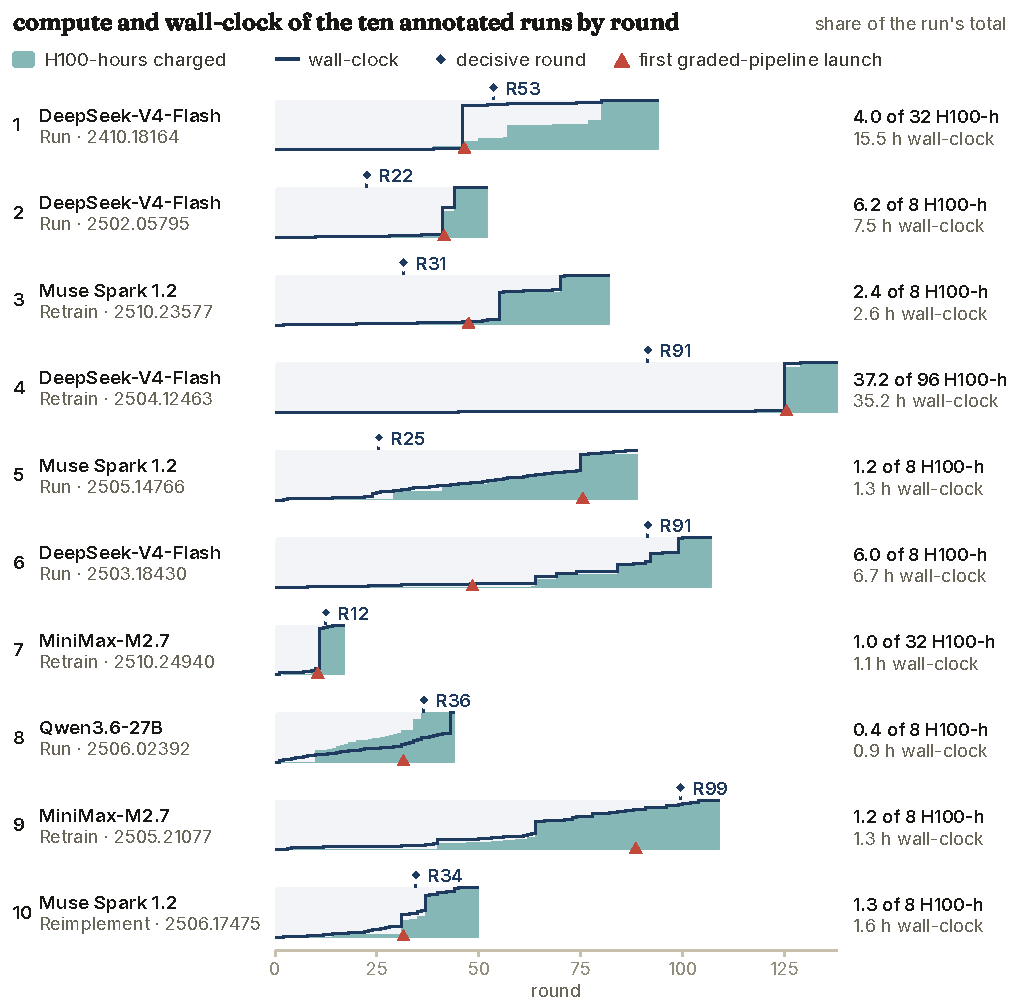
\includegraphics[width=\textwidth]{figures/app_H2_resource_trace}
\caption{Compute charged and wall-clock elapsed by round for the ten
annotated runs, each as a share of the run's total, with the decisive round
and the first graded-pipeline launch marked.}
\label{fig:app-h2-resource-trace}
\end{figure}

\begin{figure}[htb]
\centering
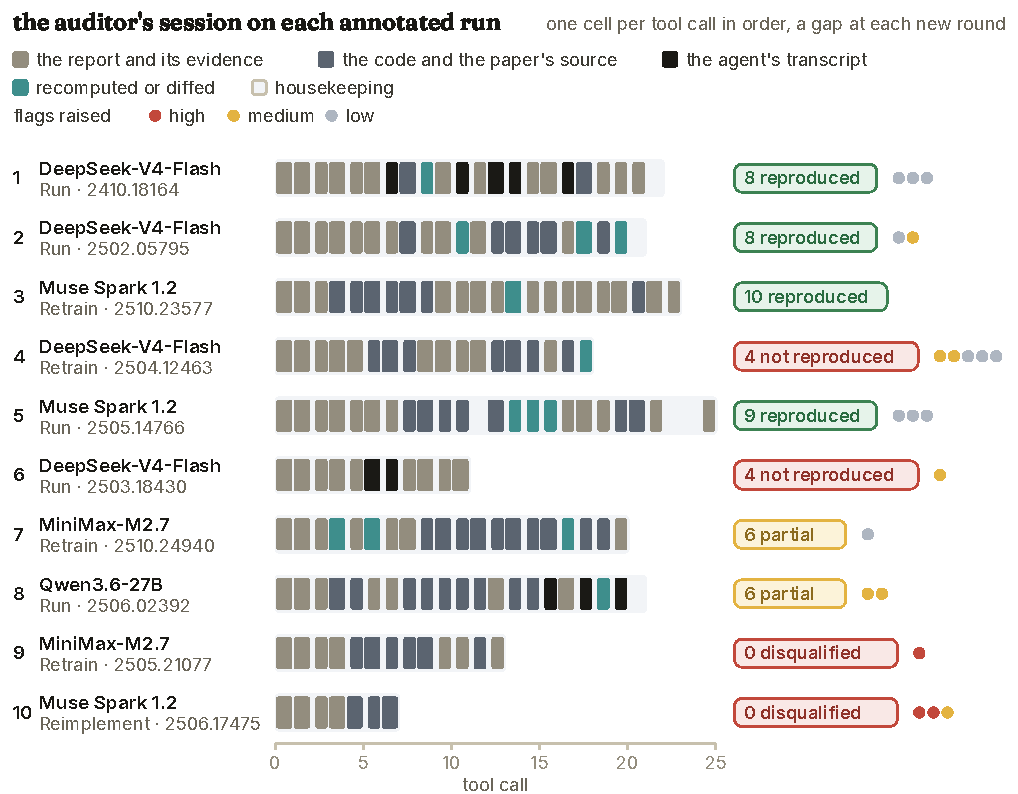
\includegraphics[width=\textwidth]{figures/app_H2_auditor_trace}
\caption{The auditor's session on each of the ten annotated runs, one cell
per tool call in order and colored by what it opened or ran, with the pinned
verdict and the flags it raised.}
\label{fig:app-h2-auditor-trace}
\end{figure}
  % resource and auditor traces of the ten runs

\FloatBarrier  % run cards stay inside this appendix
\renewcommand{\bottomfraction}{0.3}
\renewcommand{\floatpagefraction}{0.5}
